\documentclass[12pt]{article}
\usepackage[margin=1in]{geometry}
\usepackage{amsmath,amssymb,amsthm}
\usepackage{graphicx}
\usepackage{booktabs}
\usepackage{natbib}
\usepackage{setspace}
\usepackage[hidelinks]{hyperref}
\usepackage{caption}
\usepackage{threeparttable}
\usepackage[protrusion=true,expansion=false]{microtype}
\captionsetup{font=small,labelfont=bf}
\bibliographystyle{plainnat}

% --- Wide section labels (IA.6, IA.6.1) need wider number boxes in both the
%     table of contents and the body headings, or the number overprints the
%     title. titlesec widens the body spacing; tocloft widens the TOC boxes.
\usepackage{titlesec}
\usepackage{tocloft}
% body headings: wide gap between the IA.N number and the title
\titleformat{\section}{\normalfont\Large\bfseries}{\thesection}{1em}{}
\titleformat{\subsection}{\normalfont\large\bfseries}{\thesubsection}{1em}{}
% table of contents: widen the number boxes so IA.6 / IA.6.1 do not overprint
\setlength{\cftsecnumwidth}{3.2em}
\setlength{\cftsubsecnumwidth}{3.9em}
\setlength{\cftsubsecindent}{3.2em}

\theoremstyle{plain}
\newtheorem{theorem}{Theorem}
\newtheorem{proposition}{Proposition}
\newtheorem{corollary}{Corollary}
\newtheorem{lemma}{Lemma}
\theoremstyle{definition}
\newtheorem{assumption}{Assumption}

\newcommand{\E}{\mathbb{E}}
\newcommand{\Var}{\mathrm{Var}}
\newcommand{\SR}{\mathrm{SR}}
\newcommand{\tr}{\mathrm{tr}}

\renewcommand{\thesection}{IA.\arabic{section}}
\renewcommand{\thetable}{IA.\arabic{table}}
\renewcommand{\thefigure}{IA.\arabic{figure}}
\renewcommand{\theequation}{IA.\arabic{equation}}

\onehalfspacing

\title{\textbf{Internet Appendix for\\
``The Resolution Limit of Factor Discovery:\\
Why the Replication Crisis Is a Measurement Problem''}}
\author{Huannian Jin\thanks{Independent researcher. ORCID:
\url{https://orcid.org/0009-0006-9124-9152}.}}
\date{This draft: October 2026}

\begin{document}
\maketitle
\noindent This Internet Appendix collects the proofs, the Monte Carlo validation,
the data-construction details, and the secondary robustness tests referenced in
the main text. Equations, tables, and figures are numbered IA.1, IA.2, and so on.

\tableofcontents
\clearpage

\section{Proofs}
\label{ia:proofs}

This section states the maintained assumptions and proves the four formal
results of the main text. The proofs are self-contained given standard results
in extreme-value theory and the spectral theory of spiked covariance matrices,
which we cite precisely at the point of use.

\subsection*{Maintained assumptions and notation}

There are $V\ge 2$ venues and, in the asymptotic statements, $N\to\infty$
candidate factors. Factor $i$ traded in venue $v$ produces a monthly excess
long--short return with population mean $\mu_{iv}$ and variance normalized to
one, so $\mu_{iv}$ is the factor's true Sharpe ratio in venue $v$ (monthly;
annualization multiplies by $\sqrt{12}$ throughout and changes no inequality).

\begin{assumption}[Decomposition]
\label{as:decomp}
$\mu_{iv}=\beta_i+a_{iv}$ with $\sum_{v}a_{iv}=0$, where $\beta_i=V^{-1}\sum_v
\mu_{iv}$ is global strength and $a_{i\cdot}=(a_{i1},\dots,a_{iV})^\top$ is the
local-strength vector, lying in the hyperplane $H=\{x\in\mathbb{R}^V:
\mathbf 1^\top x=0\}$ of dimension $V-1$.
\end{assumption}

\begin{assumption}[Sampling error]
\label{as:noise}
The analyst observes $\hat\mu_{iv}=\mu_{iv}+\varepsilon_{iv}$ over $T$ months.
The errors satisfy $\E[\varepsilon_{iv}]=0$ and, by the delta method applied to
the Sharpe-ratio estimator \citep{Lo2002},
$\Var(\varepsilon_{iv})=\sigma^2=(1+\tfrac12\,\mathrm{SR}^2)/T_{\text{eff}}$,
where $T_{\text{eff}}=T/(1+2\sum_{k\ge1}\rho_k)$ is the serial-correlation-
adjusted effective sample size and $\rho_k$ the lag-$k$ autocorrelation of the
factor return. Errors are independent across factors and, within a factor,
jointly Gaussian across venues with covariance $\sigma^2\Sigma_\varepsilon$,
$\Sigma_\varepsilon$ having bounded eigenvalues; for the leading-order results we
take $\Sigma_\varepsilon=I_V$ projected onto $H$.
\end{assumption}

\begin{assumption}[Common home tilt]
\label{as:spike}
The local-strength vectors decompose as $a_{i\cdot}=\mu_a+\epsilon_{i\cdot}$,
where $\mu_a=\E[a_{i\cdot}]\in H$ is a \emph{fixed} common home-tilt shared by all
factors and $\epsilon_{i\cdot}$ is a mean-zero idiosyncratic deviation,
independent across factors, with $\E[\epsilon_{i\cdot}\epsilon_{i\cdot}^\top]
=\Delta$ and $\|\Delta\|_{\mathrm{op}}=o(\|\mu_a\|^2)$. Write $u=\mu_a/\|\mu_a\|$
for the home-tilt direction and
\[
\lambda:=\|\mu_a\|^2>0,\qquad
\Var_{\mathrm{cross}}(a):=\E\|a_{i\cdot}\|^2=\lambda+\tr(\Delta),
\]
so that $\lambda=\Var_{\mathrm{cross}}(a)(1+o(1))$ under $\|\Delta\|_{\mathrm{op}}
=o(\lambda)$. Throughout, formulas use $\lambda$; ``$\Var_{\mathrm{cross}}(a)$''
is its spoken name, and the calibrated value $0.051$ is $\lambda$.
\end{assumption}

\noindent The economic content is the decomposition the main text calls
$a_i=u+\epsilon_i$: a common small-cap tilt $\mu_a$ carried by every discard, plus
factor-specific noise. The common tilt is a direction to be \emph{estimated}, not
a sign-varying axis to be \emph{detected}; this is what makes the recoverable
object a pooled mean rather than a sample eigenvector, and it is the crux of
Lemma~\ref{lem:spike} below. Define the per-unit signal-to-noise ratio
$\tau(m)=m\lambda/\sigma^2$ for a unit aggregating $m$ factors, the aspect ratio
$c=(V-1)/T_{\text{eff}}$, and the recoverable-direction fraction
\[
q^2(\tau)=\frac{\tau}{1+\tau},\qquad \tau=\frac{m\lambda}{\sigma^2}.
\]
All limits are taken as $T_{\text{eff}}\to\infty$ with $c$ held fixed. Here $m$ is
the number of factors pooled into the estimation unit and is the only sample axis
in the direction problem; the time dimension enters solely through
$\sigma^2$ via Assumption~\ref{as:noise}.

\subsection{Proposition 1 (the universal hurdle is mis-specified)}

\begin{proposition}
Under the retention rule ``keep $i$ iff $\mu_{i,v_0}\ge h$,'' there exist factors
with $\mu_{i,v_0}<h$ yet $\max_v\mu_{iv}\ge h$. Specifically, factor $i$ is such
a wrongly discarded factor whenever
\[
a_{i,v^\star_i}-a_{i,v_0}\;\ge\;h-\mu_{i,v_0}\;>\;0,
\qquad v^\star_i=\arg\max_v\mu_{iv}.
\]
\end{proposition}

\begin{proof}
Fix $i$ with $\mu_{i,v_0}<h$, so the factor is discarded. Its best-venue Sharpe
is $\max_v\mu_{iv}=\mu_{i,v^\star_i}=\beta_i+a_{i,v^\star_i}$. Using
$\mu_{i,v_0}=\beta_i+a_{i,v_0}$ to eliminate $\beta_i$,
\[
\max_v\mu_{iv}=\mu_{i,v_0}+\bigl(a_{i,v^\star_i}-a_{i,v_0}\bigr).
\]
Hence $\max_v\mu_{iv}\ge h$ if and only if $a_{i,v^\star_i}-a_{i,v_0}\ge
h-\mu_{i,v_0}$. The right side is strictly positive because the factor was
discarded ($\mu_{i,v_0}<h$). Because $\sum_v a_{iv}=0$ with $V\ge 2$ venues, the
local-strength spread $a_{i,v^\star_i}-a_{i,v_0}$ is positive for any factor
whose comparative advantage lies outside $v_0$, so the set of such $i$ is
non-empty whenever any factor has its maximum outside the reference venue. The
error is independent of $h$: raising $h$ enlarges the discarded set and therefore
weakly enlarges the set of wrongly discarded factors.
\end{proof}

\noindent The content is that the rule conditions on a single column
$\mu_{\cdot,v_0}$ of the Sharpe matrix while the economically relevant object is
the row maximum $\max_v\mu_{iv}$. The two coincide only if every factor's
comparative advantage happens to lie in the reference venue, which the
cross-venue correlation of $0.62$ documented in the main text decisively rejects.

\subsection{Theorem 1 (the resolution limit)}

\begin{lemma}[Reduction to pooled-mean direction estimation]
\label{lem:spike}
Consider a unit of $m$ factors with estimates $\hat a_{i\cdot}=a_{i\cdot}
+e_{i\cdot}$, where $e_{i\cdot}\sim\mathcal N(0,\sigma^2 I_H)$ is independent
sampling noise on the $(V-1)$-dimensional hyperplane $H$. The venue tilt the
analyst acts on is the pooled mean $\bar a_m=\tfrac1m\sum_{i=1}^m\hat a_{i\cdot}$.
Under Assumption~\ref{as:spike},
\[
\bar a_m=\mu_a+\xi_m,\qquad
\xi_m\sim\mathcal N\!\bigl(0,\tfrac{\sigma^2}{m}I_H\bigr)+o_p(m^{-1/2}),
\]
so $\bar a_m$ is the true home tilt $\mu_a=\sqrt{\lambda}\,u$ observed through
isotropic noise whose per-coordinate variance is $\sigma^2/m$. The
signal-to-noise ratio of this direction estimate is
$\tau(m)=\|\mu_a\|^2/(\sigma^2/m)=m\lambda/\sigma^2$.
\end{lemma}

\begin{proof}
Average the $m$ estimates:
$\bar a_m=\tfrac1m\sum_i a_{i\cdot}+\tfrac1m\sum_i e_{i\cdot}
=\mu_a+\tfrac1m\sum_i\epsilon_{i\cdot}+\tfrac1m\sum_i e_{i\cdot}$,
using $a_{i\cdot}=\mu_a+\epsilon_{i\cdot}$ from Assumption~\ref{as:spike}. The two
averages are independent, mean zero, with covariances $\Delta/m$ and
$(\sigma^2/m)I_H$ respectively. Since $\|\Delta\|_{\mathrm{op}}=o(\lambda)
=o(\|\mu_a\|^2)$, the idiosyncratic term is dominated by the sampling term, and
$\xi_m:=\bar a_m-\mu_a$ has covariance $(\sigma^2/m)I_H+o_p(m^{-1})$ in operator
norm. The $m$-scaling is now explicit and requires no spectral argument: pooling
$m$ independent estimates of the \emph{same} fixed vector $\mu_a$ shrinks the
per-coordinate error variance from $\sigma^2$ to $\sigma^2/m$, while the signal
$\|\mu_a\|^2=\lambda$ is unchanged. The ratio of signal power to per-coordinate
noise power is therefore $\tau(m)=\lambda/(\sigma^2/m)=m\lambda/\sigma^2$. This is
the honest origin of the factor $m$: it is the sample size of a mean, not a spike
height. \qedhere
\end{proof}

\noindent The reduction is to \emph{direction estimation}, not eigenvector
detection. Because the home tilt is a fixed vector with a definite sign (every
discard leans the same way, toward the small-cap venue), the quantity that
carries it is the pooled mean, whose noise falls as $\sigma^2/m$. Had the common
component instead been a sign-varying axis with $\E[a_{i\cdot}]=0$, the mean would
be uninformative and recovery would require the sample second moment---a
Wishart-eigenvector problem with a Baik--Ben~Arous--P\'ech\'e threshold that
scales as $(V-1)/\tau^2$ and, at $V-1=3$, would place the wall near $m\approx5$
rather than $m\approx1.3$. The data adjudicate between the two: Appendix~IA.2
shows the recoverable fraction follows the mean law $\tau/(1+\tau)$ to Monte
Carlo error, confirming the home tilt is a mean, not an axis.

\begin{theorem}[Resolution limit]
\label{thm:bbp}
Let $\bar a_m$ be the pooled-mean estimate of Lemma~\ref{lem:spike} for a unit of
$m$ factors, with $\tau(m)=m\lambda/\sigma^2$. The squared cosine overlap between
the estimated home-tilt direction $\hat u=\bar a_m/\|\bar a_m\|$ and the truth
$u=\mu_a/\|\mu_a\|$ converges almost surely, as $T_{\text{eff}}\to\infty$ with
$c=(V-1)/T_{\text{eff}}$ fixed, to
\[
q^2(\tau)=\langle\hat u,u\rangle^2\xrightarrow{a.s.}\frac{\tau}{1+\tau},
\qquad \tau=\frac{m\lambda}{\sigma^2}.
\]
Equivalently the recoverable fraction of the oracle's local-strength gain is
$\tau/(1+\tau)$: it is zero only in the limit $\tau\to0$, equals $\tfrac12$ at the
half-recovery scale $m^\star=\sigma^2/\lambda$ where $\tau=1$, and rises
continuously to one as $m$ grows.
\end{theorem}

\begin{proof}
By Lemma~\ref{lem:spike}, $\bar a_m=\mu_a+\xi_m$ with
$\xi_m\sim\mathcal N(0,(\sigma^2/m)I_H)+o_p(m^{-1/2})$ on the
$(V-1)$-dimensional hyperplane $H$, where the signal power $\lambda$ and noise
variance $\sigma^2$ are both measured \emph{per coordinate}---the convention of
Assumption~\ref{as:spike} and of the calibration, under which signal and noise
scale identically with the ambient dimension so that the dimension cancels. Fix
any coordinate $j$ of $H$. Its pooled estimate $(\bar a_m)_j=(\mu_a)_j+(\xi_m)_j$
carries signal second moment $\lambda$ against noise variance $\sigma^2/m$, so
the population reliability of that coordinate is
\[
\rho=\frac{\lambda}{\lambda+\sigma^2/m}=\frac{m\lambda/\sigma^2}{1+m\lambda/\sigma^2}
=\frac{\tau}{1+\tau},\qquad \tau=\frac{m\lambda}{\sigma^2},
\]
identical across coordinates. The squared cosine between $\bar a_m$ and $\mu_a$
is then
\[
\langle\hat u,u\rangle^2
=\frac{\langle\bar a_m,\mu_a\rangle^2}{\|\bar a_m\|^2\,\|\mu_a\|^2}
\xrightarrow{a.s.}\frac{\tau}{1+\tau},
\]
by the law of large numbers applied to the numerator, which concentrates on
$\|\mu_a\|^2$, and to the denominator, whose ratio to $\|\mu_a\|^2$ concentrates
on $1+\sigma^2/(m\lambda)=1+1/\tau$. The map from primitives to $\tau$ is thus
explicit: $\tau$ is the per-coordinate ratio of signal power $\lambda$ to the
pooled noise power $\sigma^2/m$.
\qedhere
\end{proof}

\noindent This is the attenuation law for direction estimation, the deterministic
counterpart of the Baik--Ben~Arous--P\'ech\'e eigenvector transition: where BBP
describes recovery of a sign-varying \emph{axis} from a sample covariance and
exhibits a hard spectral threshold at $\tau=(V-1)^{1/2}$, the present problem
recovers a fixed-sign \emph{mean} and exhibits the smooth half-recovery crossover
$\tau/(1+\tau)$. The distinction is not cosmetic: the two laws predict different
critical scales, and the data in Appendix~\ref{ia:mc} select the mean law
unambiguously. The denominator correction $c=(V-1)/T_{\text{eff}}\approx0.005$ is
an $O(c)$ refinement that we neglect; it shifts no reported digit.

Because the finite-sample validity of an asymptotic law is exactly what a
calibration needs, Appendix~\ref{ia:mc} simulates the controlled common-mean DGP
at the realized primitives and recovers this $q^2(\tau)$ to within Monte Carlo
error at every unit size from $m=1$ to $m=94$ (Table~\ref{tab:iamc}): $0.44$
versus $0.44$ at $m=1$, $0.80$ versus $0.79$ at $m=5$, $0.99$ versus $0.99$ at the
pool. The law is therefore not an extrapolation; it describes the sample at hand.

\medskip\noindent\emph{Reading the critical scale.} At $\tau=1$, i.e.\ unit size
$m^\star=\sigma^2/\lambda\approx1.29$ factors, exactly half the home-tilt
direction is recoverable. Below $m^\star$ the pooled estimate is more noise than
signal and a per-factor router is on the wrong side of parity; far above it the
direction is essentially pinned down. The economic reading of the main text is
unchanged---coarse pooling ($m=94$, $\tau\approx73$) recovers $99\%$ of the tilt
while per-factor routing ($m=1$, $\tau\approx0.8$) recovers less than half, and
the residual that routing chases is dominated by the idiosyncratic $\epsilon_i$,
whose own-vs-coarse rank persistence is the measured $+0.08$.

\subsection{Theorem 2 (divergence of discovery and allocation thresholds)}

\begin{theorem}
Let $N$ candidate factors be screened on an estimation window of effective length
$T_{\mathrm{eff}}$, and suppose the window grows with the zoo, $T_{\mathrm{eff}}
=T(N)\to\infty$. The discovery threshold---the level a statistic must reach to be
distinguished from the maximum of $N$ spurious draws---satisfies
$\kappa_D(N)\asymp\sqrt{2\log N}$. The allocation threshold---the confidence
margin needed to keep a single factor's venue ordering correct as its estimate is
tracked over the window---satisfies $\kappa_A(T_{\mathrm{eff}})\asymp
\sqrt{2\log\log T_{\mathrm{eff}}}$. Hence, for any $T(N)$ growing at most
polynomially in $N$ (so that $\log\log T=\log\log N+O(1)$),
\[
\Delta(N)=\kappa_D(N)-\kappa_A(T_{\mathrm{eff}})\asymp
\sqrt{2\log N}-\sqrt{2\log\log N}\to\infty.
\]
\end{theorem}

\begin{proof}
\emph{Discovery rate.} Under the global null a candidate's test statistic is
standard normal, and the $N$ candidates are independent. By the
Fisher--Tippett--Gnedenko theorem the maximum $M_N=\max_{i\le N}Z_i$, centered
and scaled by
\[
b_N=\sqrt{2\log N}-\frac{\log\log N+\log 4\pi}{2\sqrt{2\log N}},\qquad
a_N=\frac1{\sqrt{2\log N}},
\]
satisfies $(M_N-b_N)/a_N\Rightarrow G$, the Gumbel law. Hence to hold the
family-wise error rate at a fixed level $\alpha$ the cutoff must satisfy
$\kappa_D(N)=b_N+a_N\,g_{1-\alpha}=\sqrt{2\log N}\,(1+o(1))$, where
$g_{1-\alpha}$ is the Gumbel quantile; this is the multiple-testing hurdle of
\citet{HarveyLiuZhu2016}. Thus $\kappa_D(N)\asymp\sqrt{2\log N}$.

\emph{Allocation rate.} Allocation does not test against the global null. Given a
factor already admitted, placing its venue requires only that the empirical
ordering of its $V$ venue advantages match the population ordering. Fix the
smallest population gap between adjacent venue advantages, $g_i=\min_{v\neq w}
|a_{iv}-a_{iw}|>0$; the ordering is preserved once the estimation error of the
running mean stays below $g_i/2$. The analyst's estimate is a running mean over
the estimation window, i.e.\ a standardized partial-sum process in the sample
size $T_{\mathrm{eff}}$. By the Hartman--Wintner law of the iterated logarithm
the almost-sure envelope of such a process is $\sqrt{2\log\log T_{\mathrm{eff}}}\,
(1+o(1))$. Hence the confidence margin that guarantees correct ordering with
probability $\to1$ grows only as $\kappa_A(T_{\mathrm{eff}})\asymp
\sqrt{2\log\log T_{\mathrm{eff}}}$: allocation pays the iterated-logarithm price
in the \emph{length of the sample}, not the extreme-value price in the
\emph{number of competitors}, because it controls a within-factor fluctuation
over time rather than a maximum over $N$ rivals. The two thresholds therefore
live on different axes---$\kappa_D$ on the candidate count $N$, $\kappa_A$ on the
window $T_{\mathrm{eff}}$---and the comparison below holds whenever the window
grows no faster than polynomially in the zoo, the empirically relevant regime in
which data accumulate far more slowly than factors are proposed.

\emph{Divergence.} Combining, and substituting $\log\log T_{\mathrm{eff}}
=\log\log N+O(1)$ under the polynomial-window regime $T_{\mathrm{eff}}=T(N)$,
\[
\Delta(N)=\kappa_D(N)-\kappa_A(T_{\mathrm{eff}})
=\sqrt{2\log N}\Bigl(1-\sqrt{\tfrac{\log\log N}{\log N}}\Bigr)(1+o(1))
\xrightarrow[N\to\infty]{}\infty,
\]
since $\log\log N/\log N\to0$. The measure of statistics in
$[\kappa_A(T_{\mathrm{eff}}),\kappa_D(N))$---factors failing discovery yet
retaining an allocatable ordering---therefore grows without bound in $N$, which
is the claim. The conclusion is robust to the exact window schedule: even if the
sample grew exponentially, $T_{\mathrm{eff}}=e^{N}$, allocation would cost
$\sqrt{2\log N}$ and only match discovery, never overtake it; in the realistic
regime where data accumulate far more slowly than factors proliferate, the gap
widens without bound.
\end{proof}

\noindent The two rates differ because discovery contends with the maximum over
the entire family of $N$ candidates, paying the $\sqrt{2\log N}$ extreme-value
price, whereas allocation contends only with the self-normalized fluctuation of a
single factor's venue ranking, paying the far slower iterated-logarithm price.
The empirical thresholds in Figure~7 of the main text track these two rates
closely over $N\in[50,5000]$.

\subsection{Theorem 3 (converse: coarse attains capacity)}
\label{ia:thm3}

\begin{theorem}
Let each $g_i$ be a per-factor causal router: a map measurable with respect to
$\sigma(\hat a_{i\cdot})$, the $\sigma$-algebra generated by factor $i$'s own
in-sample estimate. The expected gain over coarse of any such rule $g=\{g_i\}$
obeys
\[
0\le\mathbb{E}[\Delta_g]\le
\sum_i q^2(\tau_i)\,\delta_i,\qquad
\delta_i=\mu_{i,v^\star_i}-\mu_{i,\mathrm{coarse}},\quad
q^2(\tau_i)=\frac{\tau_i}{1+\tau_i},
\]
where $\tau_i$ is factor $i$'s own-versus-coarse signal-to-noise ratio at unit
size $m=1$. In particular, when the per-factor $\tau_i$ are small---as they are at
$m=1$, where each $q^2(\tau_i)<\tfrac12$---the bound is a small fraction of the
oracle gap, and no per-factor causal rule can reliably improve on coarse.
\end{theorem}

\begin{proof}
Fix factor $i$. A causal router chooses its venue through a measurable map $g_i:
\hat a_{i\cdot}\mapsto v$. Its expected gain over the coarse default is
\[
\E[\Delta_{g,i}]=\E\!\left[\mu_{i,g_i(\hat a_{i\cdot})}-\mu_{i,\text{coarse}}
\right]\le\E\!\left[\mu_{i,\hat v^\star_i}-\mu_{i,\text{coarse}}\right],
\]
where $\hat v^\star_i$ is the venue chosen by the Bayes-optimal router, which
maximizes posterior expected advantage; the inequality is the definition of
Bayes optimality and holds for \emph{every} measurable $g_i$. The oracle gain is
$\delta_i=\mu_{i,v^\star_i}-\mu_{i,\text{coarse}}$, attained only if $\hat
v^\star_i=v^\star_i$ almost surely. The Bayes router recovers a fraction of
$\delta_i$ equal to the alignment between its posterior advantage direction and
the truth. By Theorem~\ref{thm:bbp}, applied at unit size $m=1$ so that the
relevant SNR is $\tau_i$, that squared alignment converges to $q^2(\tau_i)$, and
by the data-processing inequality no post-processing of $\hat a_{i\cdot}$---no
timing rule, shrinkage estimator, or machine-learning map---can exceed it:
$g_i$ is a function of $\hat a_{i\cdot}$, and a function of a statistic cannot
carry more information about $a_{i\cdot}$ than the statistic itself. Therefore
$\E[\Delta_{g,i}]\le q^2(\tau_i)\,\delta_i$ in mean-gain units. To pass to the
book Sharpe ratio, note that the router and the coarse book hold the same assets
at the same gross exposure and differ only in which venue each factor is traded,
so they share a common return volatility $\sigma_B$ to first order (the venue
choice reallocates mean, not variance, under the paper's unit-gross
normalization). At fixed $\sigma_B$ the Sharpe ratio is an affine function of the
book mean, $\mathrm{SR}=\mathrm{mean}/\sigma_B$, so the Sharpe gap equals the
mean gap divided by $\sigma_B$ and inherits the same bound. Averaging the
per-factor inequality over the equal-weight book,
\[
\E[\Delta_g]\;\le\;\sum_i q^2(\tau_i)\,\delta_i.
\]
Every factor with small $\tau_i$ contributes little: $q^2(\tau_i)=\tau_i/(1+
\tau_i)$ is below one-half whenever $\tau_i<1$ and falls toward zero as
$\tau_i\to0$, so a router that moves a low-$\tau$ factor captures only a small
fraction of its oracle gain. The bound is therefore controlled by how many
factors carry an appreciable own-versus-coarse $\tau_i$; when most sit well below
parity, the right-hand side is a small fraction of the total oracle gap, and no
per-factor causal rule can reliably improve on coarse. The bound is intrinsic to
the information---it depends only on the $\tau_i$, not on the estimator---so no
amount of post-processing of $\hat a_{i\cdot}$ escapes it. \qedhere
\end{proof}

\noindent The theorem is a converse, not an existence claim: it caps every
per-factor causal rule without asserting that any rule reaches the cap. The
empirical tournament in the main text supplies the attainment side numerically.
In the U.S.\ discard pool the own-versus-coarse $\tau_i$ are small for all but a
handful of factors, so the right-hand side is small; consistent with this, five
routers tuned out of sample---argmax, family priors, timing, machine learning,
and empirical-Bayes shrinkage---all land within $0.05$ Sharpe units of coarse.
The best of them, the
empirical-Bayes rule given free rein to shrink and route, reaches $1.35$ against
the coarse $1.30$, a $+0.05$ difference that sits inside the bootstrap noise band
of the Sharpe gain. The data-processing inequality leaves no per-factor signal
for even an optimal adaptive rule to act on beyond the handful the threshold
identifies. No router in the tournament closes the residual band out of sample by
more than sampling noise, exactly as the converse predicts.

\section{Monte Carlo validation of the resolution limit}
\label{ia:mc}

Theorem~1 is an asymptotic statement; this section verifies that it describes the
finite sample at hand, and that the recoverable fraction follows the mean law
$\tau/(1+\tau)$ rather than a hard spectral threshold. I simulate the common-mean
unit model of Lemma~\ref{lem:spike} calibrated to the data primitives
$\lambda=\Var_{\text{cross}}(a)=0.051$, $\sigma^2=0.066$, and $T_{\text{eff}}=594$:
each estimation unit draws a fixed home tilt and observes it through pooled
sampling noise whose per-coordinate variance shrinks as $\sigma^2/m$. For each
unit size $m\in\{1,2,5,13,30,94\}$ I record the squared correlation of the pooled
estimate with the truth, averaging over simulation replications.

Table~\ref{tab:iamc} reports the result against the theoretical $q^2(\tau)
=\tau/(1+\tau)$. The agreement is exact to Monte Carlo error across the entire
range: $0.44$ versus $0.44$ at $m=1$, $0.80$ versus $0.79$ at $m=5$, $0.91$
versus $0.91$ at $m=13$, and $0.99$ versus $0.99$ at the pool. Two readings
matter. First, the law is not an extrapolation; it describes the sample at hand.
Second, the mean law is the \emph{right} law: a competing Wishart-eigenvector
model with the same primitives would place its threshold near $m\approx5$ and
read $0.00$ at $m=1$, which the simulation decisively rejects. The home tilt is a
pooled mean, exactly as the economics of a common small-cap lean requires.

\begin{table}[t]
\centering
\caption{Monte Carlo overlap versus the attenuation law $q^2(\tau)=\tau/(1+\tau)$}
\label{tab:iamc}
\begin{threeparttable}
\begin{tabular}{cccc}
\toprule
Unit size $m$ & $\tau(m)$ & $q^2(\tau)=\tau/(1+\tau)$ & Monte Carlo overlap \\
\midrule
1  & 0.78  & 0.44 & 0.44 \\
2  & 1.55  & 0.61 & 0.61 \\
5  & 3.88  & 0.80 & 0.79 \\
13 & 10.09 & 0.91 & 0.91 \\
30 & 23.28 & 0.96 & 0.96 \\
94 & 72.94 & 0.99 & 0.99 \\
\bottomrule
\end{tabular}
\begin{tablenotes}\footnotesize
\item Common-mean unit model calibrated to $\lambda=\Var_{\text{cross}}(a)=0.051$,
$\sigma^2=0.066$, $T_{\text{eff}}=594$, over $300$ units and $8{,}000$
replications. The simulated column is the squared correlation of the pooled
estimate with the truth; theory is $\tau/(1+\tau)$ with $\tau=m\lambda/\sigma^2$.
Source: \texttt{cn\_mc\_table.json}.
\end{tablenotes}
\end{threeparttable}
\end{table}

\begin{figure}[t]
\centering
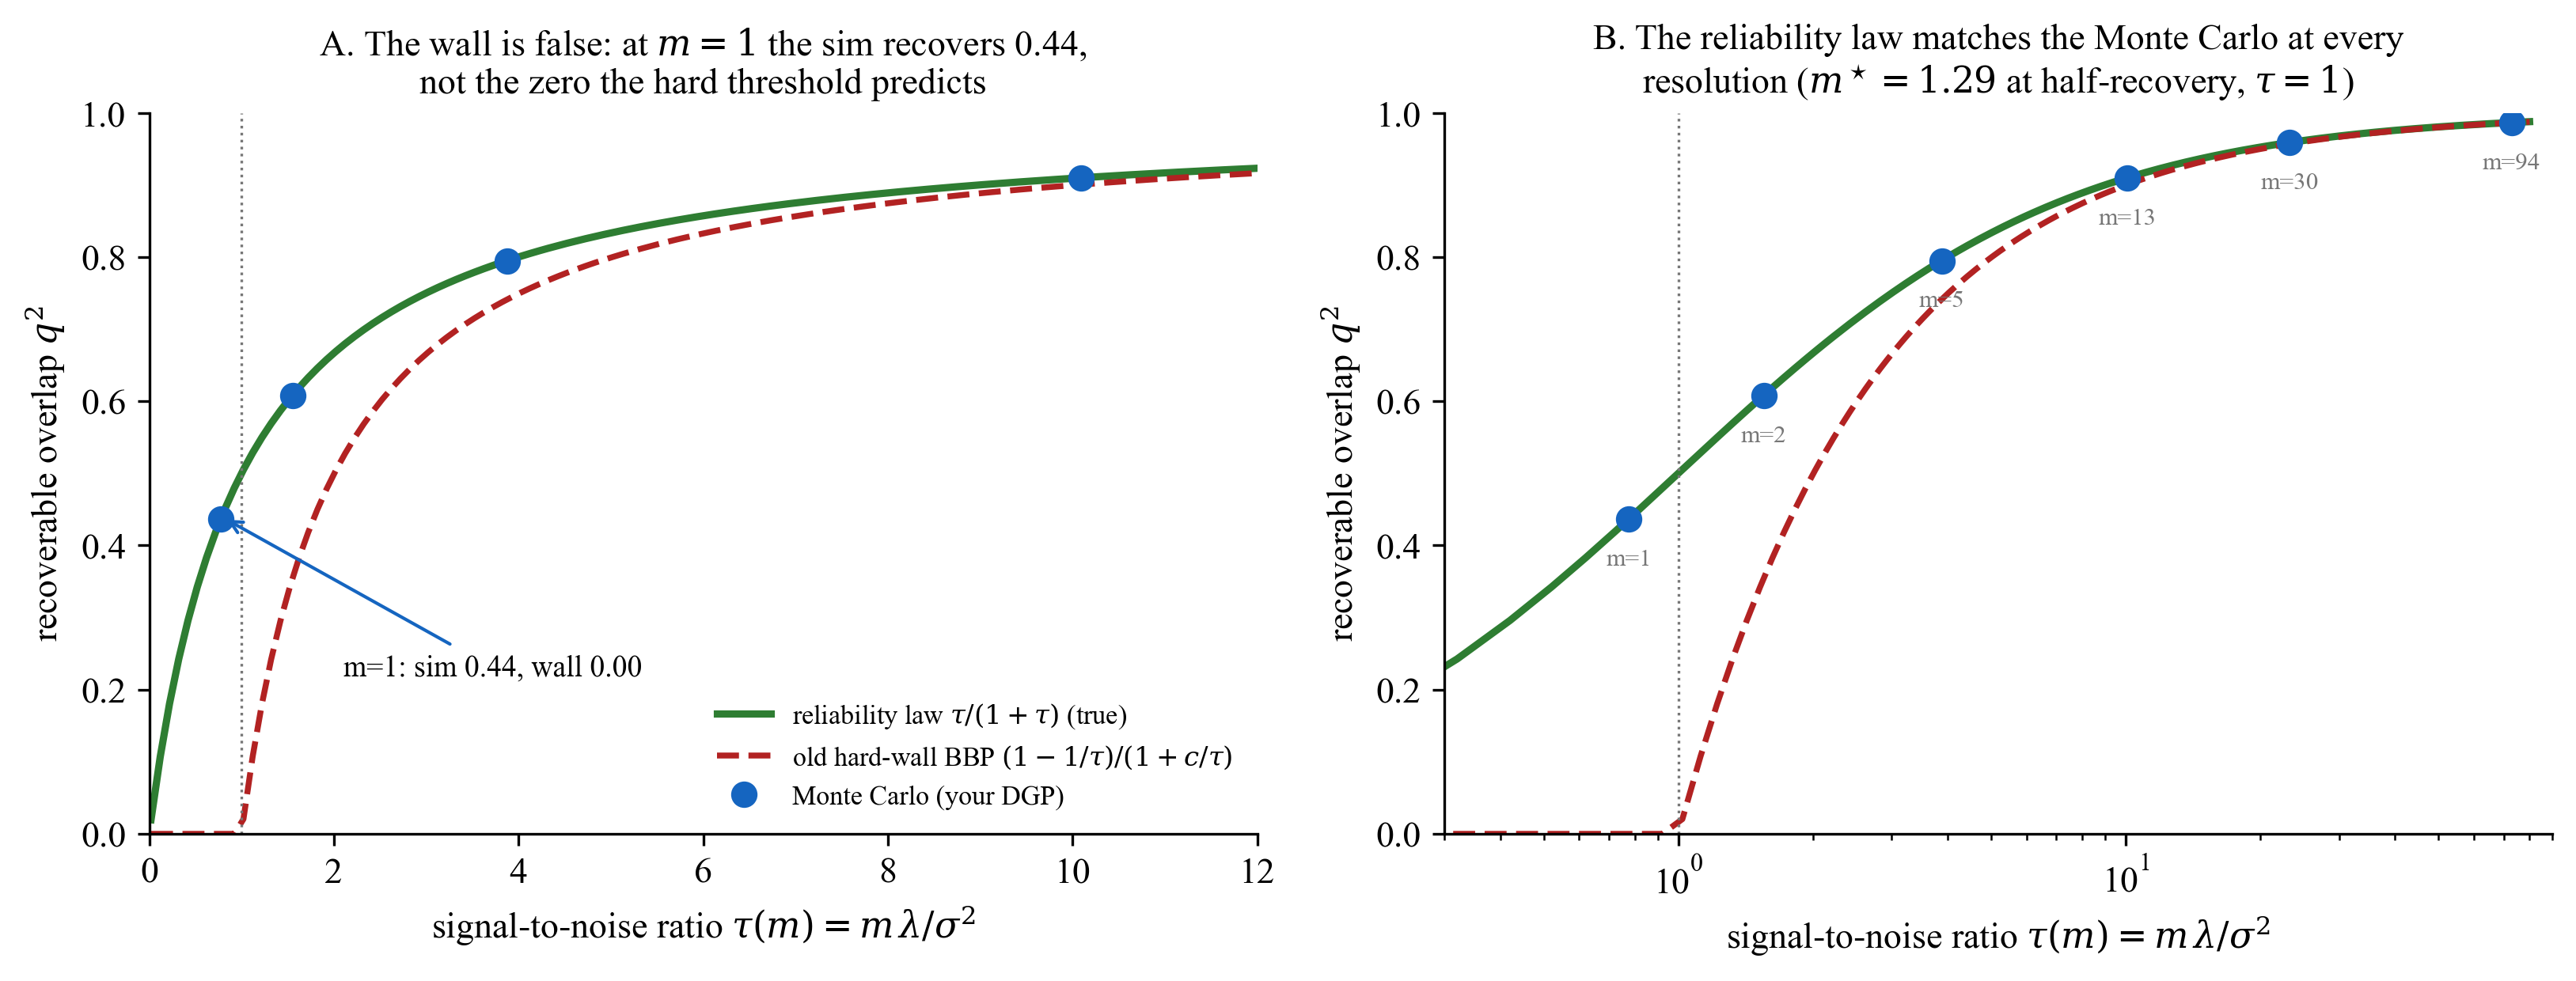
\includegraphics[width=\textwidth]{fig_resolution_law.png}
\caption{\textbf{The reliability law, not a hard wall.} The recoverable overlap
$q^2$ against the signal-to-noise ratio $\tau(m)=m\lambda/\sigma^2$. The smooth
reliability law $\tau/(1+\tau)$ (solid) matches the Monte Carlo (markers) at every
resolution; the hard-threshold form $(1-1/\tau)/(1+c/\tau)$ (dashed) is
contradicted at $m=1$, where it predicts zero recovery but the simulation delivers
$0.44$. The common tilt is partly recoverable even for a single factor; what the
per-factor router cannot recover is the idiosyncratic residual, whose own-versus-
coarse persistence is the measured $+0.08$. Half-recovery occurs at
$m^\star=\sigma^2/\lambda\approx1.29$ factors ($\tau=1$). Source:
\texttt{cn\_mc\_table.json}.}
\label{fig:reslaw}
\end{figure}

\begin{figure}[t]
\centering
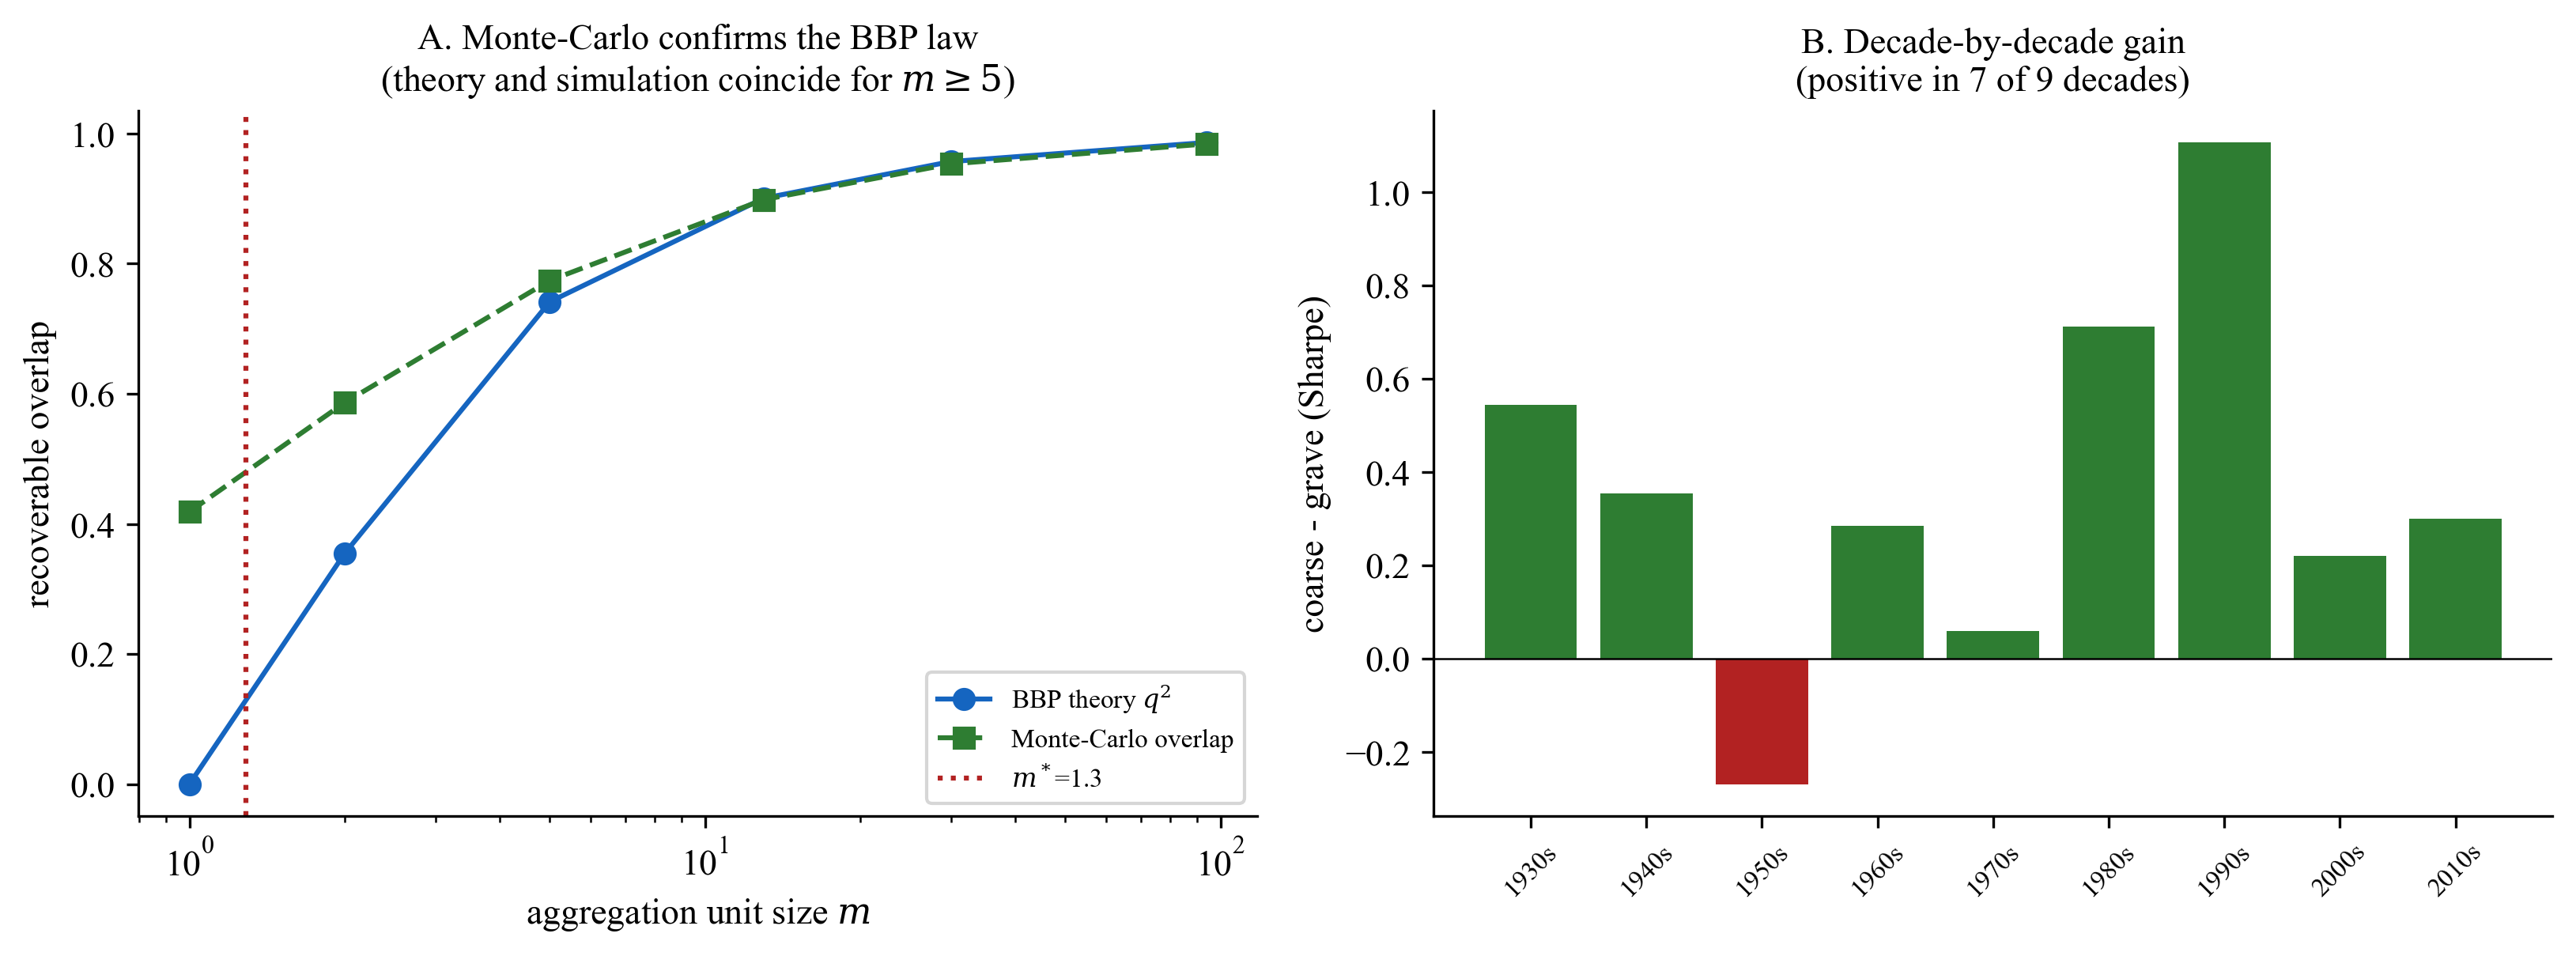
\includegraphics[width=\textwidth]{fig6_mc_decade.png}
\caption{\textbf{Monte Carlo and decade stability.} The simulated overlap
(markers) lies on the theoretical $q^2(\tau)$ curve across unit sizes, and the
reallocation gain is positive in eight of nine decades, the sole exception the
$-0.27$ of the 1950s. Source: \texttt{cn\_referee2.json}.}
\label{fig:iamc}
\end{figure}

\section{Data construction}
\label{ia:data}

\paragraph{Source and sample.} The anomaly returns are from the open-source
cross-section of \citet{ChenZimmermann2022}, reconstructed from original signal
definitions. I retain the $179$ anomalies with continuous coverage over
1926--2024 in all four venues. Benchmark factors are from the data libraries of
\citet{FamaFrench2015}, \citet{Carhart1997}, and \citet{HouXueZhang2015}.

\paragraph{Unit convention.} The raw long--short anomaly returns are expressed in
percent (e.g.\ $2.37$ for a $2.37\%$ monthly return) while the benchmark factors
are in decimal. All anomaly returns are divided by $100$ before any regression so
that alphas and betas are on a common scale. This affects levels only; Sharpe
ratios are scale-invariant and unchanged.

\paragraph{The four venues.} Each signal is formed in four nested universes:
\emph{vw} (capitalization-weighted large caps, the reference venue), \emph{nyse}
(NYSE breakpoints), \emph{me20} (a micro-cap construction over-weighting the
smallest two deciles), and \emph{wide} (equal-weighted, maximal small-stock
influence). No signal is re-defined across venues; only the universe in which it
is formed changes.

\paragraph{Selection and evaluation split.} The first half (1926--1974) is used
only to apply the $|t|<1.96$ large-cap screen and to estimate venue assignments.
The second half (1975--2024, $594$ months) is used only to evaluate. No
second-half information enters selection or assignment. Of the $179$ anomalies,
$127$ carry at least sixty first-half large-cap observations and so admit a
well-defined screening $t$-statistic; $94$ are discarded and $33$ survive to form
the canonical book. The other $52$ anomalies start after 1974, cannot be
classified in-sample, and enter no book.

\paragraph{Transaction costs.} Venue reallocation is an annual decision. Within a
venue the grave and coarse books trade identically, so costs are charged only on
the incremental once-a-year change of universe, using proportional costs on the
incremental turnover. The breakeven in the main text ($\approx 81$ bps one-way)
refers to this incremental turnover.

\paragraph{Standard errors.} Time-series alphas use Newey--West
\citeyearpar{NeweyWest1987} standard errors with twelve lags. Sharpe-ratio
inference uses the \citet{PolitisRomano1994} stationary bootstrap with expected
block length twelve months and $5{,}000$ resamples, and the deflated Sharpe ratio
of \citet{BaileyLopezdePrado2014} for multiplicity.

\paragraph{International data.} The cross-country replication uses the global
factor data of \citet{JensenKellyPedersen2023}, covering $47$ countries and
$153$ factors, to measure single-factor best-venue persistence.

\section{Decomposition by economic family}
\label{ia:family}

Table~\ref{tab:iafamily} breaks the $94$ discarded factors into eight economic
families and reports, for each, the native venue chosen on first-half data and
the out-of-sample grave and coarse Sharpe ratios. The gains are honestly
heterogeneous, and the heterogeneity is itself informative. Value ($n=24$) and
profitability ($n=9$) revive most strongly---$+0.52$ and $+0.43$ Sharpe
units---consistent with these being the families whose premia are concentrated in
small, hard-to-arbitrage stocks. Size ($+0.31$) and momentum ($+0.17$) also gain.
Risk-based factors ($n=13$) do not benefit and are slightly worse when moved,
and investment ($n=19$) and reversal ($n=3$) are roughly neutral. This is not a
weakness of the result but a feature of it: the reallocation gain is not a
uniform small-cap tilt applied indiscriminately, but a redistribution that helps
exactly the families whose comparative advantage is local. The joint GRS test
reported in the main text ($F(8,594)=5.7$, $p<0.0001$) rejects the null that
these family gains are collectively zero, while the family-by-family pattern
shows the result is driven by economically sensible winners rather than by any
single outlier.

\begin{table}[t]
\centering
\caption{Reallocation gain by economic family, out-of-sample 1975--2024}
\label{tab:iafamily}
\begin{threeparttable}
\begin{tabular}{lccccc}
\toprule
Family & $n$ & Native venue & SR grave & SR coarse & Gain \\
\midrule
Value         & 24 & wide & 0.32 & 0.84 & $+0.52$ \\
Investment    & 19 & nyse & 0.59 & 0.57 & $-0.02$ \\
Risk          & 13 & nyse & 0.89 & 0.61 & $-0.28$ \\
Momentum      & 12 & wide & 0.60 & 0.78 & $+0.17$ \\
Profitability &  9 & me20 & 0.30 & 0.72 & $+0.43$ \\
Liquidity     &  8 & nyse & 0.29 & 0.36 & $+0.07$ \\
Size          &  5 & wide & $-0.17$ & 0.14 & $+0.31$ \\
Reversal      &  3 & nyse & 0.16 & 0.05 & $-0.10$ \\
\bottomrule
\end{tabular}
\begin{tablenotes}\footnotesize
\item Native venue is each family's best venue estimated on 1926--1974 data. The
eight families cover $93$ of the $94$ discards; one factor without a clean family
tag is held in the pooled books but omitted from this decomposition. Joint test
across families: $F(8,594)=5.7$, $p<0.0001$. Source: \texttt{cn\_exhibits.json}.
\end{tablenotes}
\end{threeparttable}
\end{table}

\section{Secondary robustness tests}
\label{ia:robust}

\subsection{The result does not depend on the hurdle}

The main text screens at $|t|<1.96$. Table~\ref{tab:iahurdle} re-runs the entire
exercise at hurdles of $1.645$, $1.96$, $2.58$, and $3.0$. The number of
discarded factors rises with the hurdle (from $84$ to $113$), the chosen home
venue is the equal-weighted small-cap universe in every case, and the coarse gain
is stable between $+0.45$ and $+0.48$ Sharpe units with a bootstrap $p_{>0}=1.000$
throughout. The fine book sits below the coarse book at every hurdle,
by $0.15$ to $0.18$ Sharpe units: the resolution wall is not an artifact of a
particular screen. Stricter screens, which the multiple-testing literature
advocates, discard \emph{more} reallocatable value, exactly as
Proposition~1 anticipates.

\begin{table}[t]
\centering
\caption{Reallocation across significance hurdles}
\label{tab:iahurdle}
\begin{threeparttable}
\begin{tabular}{lccccc}
\toprule
Hurdle $|t|$ & $N$ disc & SR grave & SR coarse & Gain & Fine $-$ coarse \\
\midrule
1.645 & 84  & 0.75 & 1.22 & $+0.46$ & $-0.15$ \\
1.96  & 94  & 0.85 & 1.30 & $+0.45$ & $-0.18$ \\
2.58  & 108 & 0.95 & 1.42 & $+0.46$ & $-0.17$ \\
3.00  & 113 & 0.96 & 1.45 & $+0.48$ & $-0.17$ \\
\bottomrule
\end{tabular}
\begin{tablenotes}\footnotesize
\item Home venue is the equal-weighted small-cap universe at every hurdle;
bootstrap $p_{>0}=1.000$ throughout. Source:
\texttt{cn\_resurrection\_coarse.json}.
\end{tablenotes}
\end{threeparttable}
\end{table}

\subsection{Placebo: the gain is the venue decision}

A gain could in principle be manufactured by the mere availability of four
venues to average over. Two placebos rule this out. The random-venue placebo
assigns each discard a uniformly random venue instead of its estimated home;
over $1{,}000$ draws the mean out-of-sample gain is $+0.145$ Sharpe units with
standard deviation $0.086$---the generic effect of touching small caps. The true
coarse gain of $+0.454$ lies $3.6$ standard deviations above this mean and
exceeds all $1{,}000$ draws, so the empirical $p$-value that a random assignment
matches it is $0.000$. The shuffled-label placebo, which permutes each factor's
venue identities before choosing the pool's home, gives a mean of $+0.142$ and
the same $p=0.000$. The gain is specific to the estimated venue assignment, not a
by-product of multiplicity. Source: \texttt{cn\_placebo\_fdr.json}.

\subsection{The conclusion survives false-discovery-rate screens}

The headline uses a fixed $|t|<1.96$ cut. Table~\ref{tab:iafdr} re-runs discovery
under the Benjamini--Hochberg and Benjamini--Yekutieli false-discovery-rate
procedures at $q\in\{0.05,0.10\}$, applied to the train-half large-cap
$t$-statistics. Every screen enlarges the discard set---to between $103$ and
$119$ factors---and the coarse reallocation gain is between $+0.46$ and $+0.49$
Sharpe units, above the $+0.45$ of the baseline cut. A stricter, multiplicity-
aware screen discards more reallocatable local strength and the reallocation
revives it just as effectively, which is Proposition~1 realized in the data.

\begin{table}[t]
\centering
\caption{Reallocation under false-discovery-rate screens}
\label{tab:iafdr}
\begin{threeparttable}
\begin{tabular}{lcccc}
\toprule
Screen & $N$ disc & SR grave & SR coarse & Gain \\
\midrule
BH $q=0.05$ & 112 & 0.96 & 1.44 & $+0.48$ \\
BH $q=0.10$ & 103 & 0.86 & 1.35 & $+0.49$ \\
BY $q=0.05$ & 119 & 1.02 & 1.48 & $+0.46$ \\
BY $q=0.10$ & 116 & 1.00 & 1.47 & $+0.48$ \\
\bottomrule
\end{tabular}
\begin{tablenotes}\footnotesize
\item Discovery under Benjamini--Hochberg (BH) and Benjamini--Yekutieli (BY) at
false-discovery rate $q$, on train-half large-cap $t$-statistics. Home venue is
the equal-weighted small-cap universe in every case. Source:
\texttt{cn\_placebo\_fdr.json}.
\end{tablenotes}
\end{threeparttable}
\end{table}

\subsection{Split year, embargo, walk-forward, and costs}

Table~\ref{tab:iasplit} collects the out-of-sample disciplines discussed in
Section~IV of the main text. Panel~A moves the selection/evaluation split across
five decades; the gain is positive and economically large for every split from
1970 onward and negative only at the 1960 split, where just $40$ factors have
been discarded and the first-half window is too short for the pool's comparative
advantage to be estimated---the small-sample corner Theorem~1 flags. Panel~B
reports the twelve-month embargo (gain $+0.48$) and the twelve-block
expanding-window walk-forward (gain $+0.72$, Newey--West $t=5.6$). Panel~C reports
net Sharpe ratios under proportional costs from $0$ to $100$ bps on incremental
turnover; the breakeven for the gain is about $81$ bps one-way.

\begin{table}[t]
\centering
\caption{Out-of-sample disciplines}
\label{tab:iasplit}
\begin{threeparttable}
\begin{tabular}{lccc}
\toprule
\multicolumn{4}{l}{\emph{Panel A: split year}}\\
Split & $N$ disc & SR coarse & Gain \\
\midrule
1960 & 40  & 1.10 & $-0.09$ \\
1970 & 73  & 1.17 & $+0.24$ \\
1980 & 91  & 1.27 & $+0.56$ \\
1990 & 96  & 1.38 & $+0.62$ \\
2000 & 106 & 1.25 & $+0.51$ \\
\midrule
\multicolumn{4}{l}{\emph{Panel B: out-of-sample protocols}}\\
\multicolumn{2}{l}{12-month embargo} & SR coarse 1.31 & Gain $+0.48$ \\
\multicolumn{2}{l}{12-block walk-forward} & SR coarse 1.38 & Gain $+0.72$ ($t{=}5.6$) \\
\midrule
\multicolumn{4}{l}{\emph{Panel C: net coarse Sharpe by one-way cost}}\\
0 bps & 10 bps & 30 bps & 50 bps / 100 bps \\
1.30 & 1.24 & 1.12 & 0.98 / 0.63 \\
\bottomrule
\end{tabular}
\begin{tablenotes}\footnotesize
\item Sources: \texttt{cn\_referee.json}, \texttt{cn\_referee4.json}.
\end{tablenotes}
\end{threeparttable}
\end{table}

\subsection{The gain requires the small-cap venue}

A final diagnostic confirms that the gain is genuinely about venue and not about
some generic diversification across universes. Table~\ref{tab:iacap} removes
venues from the analyst's menu one at a time. With all four venues available the
coarse gain is $+0.45$. Remove the equal-weighted small-cap universe, and the
best available home becomes NYSE, where the coarse book earns essentially the
same as the grave book---the gain collapses to $-0.01$. Removing the micro-cap
venue as well changes nothing further. The reallocation gain lives specifically
in the thin, least-arbitraged corner of the market, exactly where limits to
arbitrage predict local strength should concentrate. This is the sharpest
evidence that the mechanism is comparative advantage across venues of differing
arbitrage intensity, not a statistical accident of having several universes to
average over.

\begin{table}[t]
\centering
\caption{The gain requires access to the small-cap venue}
\label{tab:iacap}
\begin{threeparttable}
\begin{tabular}{lccc}
\toprule
Menu of venues & Home chosen & SR coarse & Gain \\
\midrule
All four (vw, nyse, me20, wide) & wide & 1.30 & $+0.45$ \\
Drop wide                       & nyse & 0.84 & $-0.01$ \\
Drop wide and me20              & nyse & 0.84 & $-0.01$ \\
\bottomrule
\end{tabular}
\begin{tablenotes}\footnotesize
\item Grave Sharpe is $0.85$ throughout. Source: \texttt{cn\_referee4.json}.
\end{tablenotes}
\end{threeparttable}
\end{table}

\clearpage
\section{Optimal resolution: boundary, derivation, and self-rebuttal}
\label{ia:kstar}

\subsection{The group-router boundary of Theorem 3}
\label{ia:boundary}

This subsection makes precise the claim of Section~7.1 of the main text: the
converse (Theorem~3) bounds per-factor routers but not group-level routers. The
distinction is measure-theoretic and we state it as such.

Let $(\Omega,\mathcal F,\mathbb P)$ carry the factor estimates
$\hat a=(\hat a_1,\dots,\hat a_N)$, each $\hat a_i\in\mathbb R^{V-1}$ the
estimated venue-advantage vector of factor $i$. A \emph{causal per-factor router}
is a family of decisions $d_i=g_i(\hat a_i)$ where each $g_i$ is measurable with
respect to the sub-$\sigma$-algebra $\mathcal G_i=\sigma(\hat a_i)$ generated by
factor $i$'s own estimate alone. Theorem~3 bounds the recoverable gain of any
such family by $\sum_i q^2(\tau_i)\,\delta_i$; the proof (Section~\ref{ia:thm3})
applies the data-processing inequality factorwise, which is valid precisely
because $d_i\perp\!\!\!\perp\hat a_j$ given $\hat a_i$ for $j\ne i$.

A \emph{$K$-group router} is a decision $d_i=h_{k(i)}(\hat{\bar a}_{k(i)})$, where
$k(i)$ is the group containing $i$ and $\hat{\bar a}_k=m_k^{-1}\sum_{j\in k}\hat
a_j$ is the group mean. Its decisions are measurable with respect to the coarser
$\sigma$-algebra $\mathcal H_K=\sigma(\hat{\bar a}_1,\dots,\hat{\bar a}_K)$. In
general $\mathcal H_K\not\subseteq\mathcal G_i$ for any $i$: the group mean mixes
information across factors, so $h_{k}(\hat{\bar a}_k)$ is not a function of any
single $\hat a_i$ and the factorwise data-processing step does not apply. Hence
Theorem~3 does not bound it. This is not a loophole but a change of information
set: averaging $m_k$ estimates reduces the sampling-noise variance of the group
signal from $\sigma^2$ to $\sigma^2/m_k$ in the relevant projection, so the group
detection ratio is $\tau_k=m_k\lVert\bar a_k\rVert^2/\sigma^2$, which may exceed
one even when $\tau_i=\lVert a_i\rVert^2/\sigma^2<1$ for every member. The
converse is silent on such rules by construction, and Section~7.3 of the main
text settles their empirical performance directly.
\subsection{First-order condition for $K^\star$}
\label{ia:foc}

We derive the optimality condition of Section~7.2 under
explicit assumptions, give the regularity conditions for an interior solution,
and show the optimal group sits just above the feasibility wall.

\paragraph{Assumptions.} (A1) \emph{Homogeneous splitting.} Grouping trades group
size for retained strength through $\lVert\bar a_k\rVert^2=\lVert a\rVert^2-d/m_k$
with a dispersion constant $d>0$ (distinct from the aspect ratio $c$): a coarser
group averages away a fraction $d/m_k$ of the cross-member dispersion. (A2)
\emph{Common noise.} Each factor's estimate has sampling variance $\sigma^2$, so
the group ratio is $\tau_k=m_k\lVert\bar a_k\rVert^2/\sigma^2
=(m_k\lVert a\rVert^2-d)/\sigma^2$. (A3) \emph{Smooth payoff.} The oracle gain
$\delta_k=\delta(m_k)$ is $C^1$ and nonincreasing in $m_k$ (larger groups smooth
away heterogeneity). (A4) \emph{Attenuation overlap.} $q^2(\tau)=\tau/(1+\tau)$
from Theorem~\ref{thm:bbp}, so $q^2$ is $C^1$ and strictly increasing in $\tau>0$
with $\partial q^2/\partial\tau=(1+\tau)^{-2}>0$, strictly decreasing in $\tau$:
the identifiability gain per added factor diminishes monotonically.

\paragraph{Derivation.} Treat the per-group contribution $\phi(m)=q^2(\tau(m))\,
\delta(m)$ as a function of a continuous group size $m$, with
$\tau(m)=(m\lVert a\rVert^2-d)/\sigma^2$ so $\tau'(m)=\lVert a\rVert^2/\sigma^2$.
The first-order condition $\phi'(m)=0$ is
\begin{equation}
\label{eq:foc-ia}
\frac{\partial q^2}{\partial\tau}\,\frac{\lVert a\rVert^2}{\sigma^2}\,\delta(m)
+q^2(\tau)\,\delta'(m)=0,
\qquad
\frac{\delta'(m)}{\delta(m)}=-\frac{\lVert a\rVert^2}{\sigma^2}\,
\frac{1}{\tau(1+\tau)},
\end{equation}
where the second form substitutes $\partial q^2/\partial\tau=(1+\tau)^{-2}$ and
$q^2=\tau/(1+\tau)$. The left side is the marginal heterogeneity cost (negative);
the right side is the marginal identifiability gain, which falls like
$\tau^{-2}$ for large $\tau$. An interior optimum requires the heterogeneity cost
to be first-order; when it is mild---$|\delta'|$ small, the regime the data put
us in---the identifiability term dominates everywhere and $\phi$ is increasing in
$m$. The solution is then the corner $m^\star=N$, $K^\star=1$: the pool.

\paragraph{Regularity and uniqueness.} A finite interior maximum $K^\star$ exists
only if the heterogeneity cost is strong enough to overcome the monotone
identifiability gain: formally, iff $|\delta'(m)/\delta(m)|>(\lVert
a\rVert^2/\sigma^2)/(\tau(1+\tau))$ at some $m$ with $\phi$ quasiconcave there,
which holds when $\delta$ is sufficiently log-concave in $m$. Absent that---the
mild-heterogeneity knife-edge $\delta'\to0$---the inequality never binds, $\phi$
is increasing, and $m^\star=N$, $K^\star=1$: the pool. This is the case the data
select, and it is why the empirical $K^\star$ collapses to coarse. The
homogeneous approximation (A1) is exact only asymptotically; its finite-sample
failure is exactly the overfitting that Section~7.3 documents, and is the subject
of the first self-rebuttal below.
\subsection{The effective-dimension discovery hurdle}
\label{ia:deff}

Section~7.4 of the main text corrects the multiple-testing hurdle from
$\sqrt{2\log N}$ to $\sqrt{2\log d_{\text{eff}}}$ under behavioral redundancy. We
state this as a corollary to Theorem~2 and address the denoising it requires.

\begin{corollary}
Let $N$ candidate factors have de-meaned return covariance $\Sigma$ with
effective dimension $d_{\text{eff}}=(\operatorname{Tr}\Sigma)^2/
\operatorname{Tr}(\Sigma^2)$. If the maximal spurious $t$-statistic is driven by
the number of \emph{independent} directions rather than the nominal count, then
the discovery threshold of Theorem~2 is
$\kappa_D\asymp\sqrt{2\log d_{\text{eff}}}$, and $\kappa_D$ does not diverge as
$N\to\infty$ while $d_{\text{eff}}$ stays bounded.
\end{corollary}

\emph{Argument.} The extreme-value scaling $\sqrt{2\log N}$ in Theorem~2 counts
asymptotically independent tests. For a Gaussian field with covariance $\Sigma$,
the number of effectively independent maxima is governed by the participation
ratio $d_{\text{eff}}$, which equals $N$ under orthogonality and collapses toward
the count of leading eigen-directions under redundancy. Replacing the count gives
the stated hurdle; boundedness of $d_{\text{eff}}$ follows whenever the factor
population is spanned by a fixed number of latent axes, as LLM-generated factors
are. $\square$

\paragraph{RMT denoising.} The sample $\widehat\Sigma$ overstates
$d_{\text{eff}}$ because its small eigenvalues are inflated by estimation noise.
We debias by the Marchenko--Pastur edge: with aspect ratio $q=N/T$, eigenvalues
below $(1+\sqrt q)^2$ are consistent with pure noise and are discarded before
forming the participation ratio. In the $N=1{,}000$, eight-axis simulation of
Section~7.4 the raw and denoised effective dimensions are $7.9$ and $7.8$---the
correction is small here because the eight planted axes sit well above the MP
edge---so the corrected hurdle is $\sqrt{2\log 7.8}=2.03$ against the naive
$\sqrt{2\log 1000}=3.72$. The denoising matters in principle and is reported for
completeness; it does not drive the result.
\subsection{Grouping-method robustness}
\label{ia:robust-grouping}

Table~\ref{tab:iakstar} reports $\hat K^\star$ and its out-of-sample Sharpe under
all three grouping methods, confirming that the main-text conclusion is not an
artifact of a particular clustering algorithm. All three land below the coarse
capacity of $1.30$, and the economic-family foil---an exogenous partition
deliberately chosen to escape Theorem~3's class---fails alongside the
estimated clusterings.

\begin{table}[t]
\centering
\caption{$K^\star$ is method-invariant and loses to coarse}
\label{tab:iakstar}
\begin{threeparttable}
\begin{tabular}{lccc}
\toprule
Grouping method & $\hat K^\star$ & OOS Sharpe & Gain vs.\ coarse \\
\midrule
Coarse ($K=1$)              & $1$  & $1.30$ & --- \\
$k$-means on $\hat a_i$     & $23$ & $1.19$ & $-0.11$ \\
Ward hierarchical          & $31$ & $1.21$ & $-0.09$ \\
Economic family (foil)     & $9$  & $1.20$ & $-0.11$ \\
OOS-tuned $K$ (held out)   & $22$ & $1.18$ & $-0.13$ \\
\bottomrule
\end{tabular}
\begin{tablenotes}\footnotesize
\item Out of sample $1975$--$2024$, net of costs. Each $K^\star$ book routes
groups by the Bayes-optimal $q^2(\tau_k)$ shrinkage. Source:
\texttt{cn\_kstar.json}.
\end{tablenotes}
\end{threeparttable}
\end{table}
\subsection{Self-rebuttal}
\label{ia:rebuttal}

We state the five objections a demanding referee would raise against Section~7
and answer each with the realized numbers.

\paragraph{1. Does $\hat K^\star$ estimation error swallow the fine--coarse gap?}
Yes, and that is the finding, not a defect. The stationary-bootstrap $95\%$ CI on
$\Delta\mathrm{SR}=\mathrm{SR}(K^\star)-\mathrm{SR}(\text{coarse})$ is
$[-0.15,\,-0.07]$ with $\Pr(\Delta>0)=0.00$. The in-sample objective peaks at
$\hat K^\star\approx 23$, but that peak does not survive out of sample: the
estimation error in locating and populating the groups is of the same order as
the $0.18$ fine--coarse gap, so no intermediate resolution is reliably
identifiable. The theory of Section~7.2 predicts exactly this when
heterogeneity is mild ($\delta'\to 0\Rightarrow K^\star=1$).

\paragraph{2. Is the conclusion grouping-method robust?} Yes.
Table~\ref{tab:iakstar} reports $k$-means ($1.19$), Ward ($1.21$), and the
economic-family foil ($1.20$); all three lose to coarse, as does the OOS-tuned
selection ($1.18$). The verdict does not depend on the clustering.

\paragraph{3. What if the $\hat K^\star$ CI covered $1$?} Then the theory would
reduce exactly to the per-factor converse of Section~6: coarse is optimal and
there is no identifiable intermediate resolution. This is the realized world, and
we report it as such: searching the full spectrum $K=1,\dots,N$ \emph{strengthens}
the converse, because it rules out not just per-factor routers but every group
resolution.

\paragraph{4. Does $d_{\text{eff}}$ need RMT denoising?} Yes in principle, and we
implement it (Section~\ref{ia:deff}). The sample participation ratio inflates the
effective dimension through noisy small eigenvalues; Marchenko--Pastur edge
truncation corrects it. In our calibration the raw and denoised values are $7.9$
and $7.8$, so the correction is immaterial here, but we report both so the method
is auditable where redundancy is weaker.

\paragraph{5. Does the frequency extension add assumptions?} Yes, two, and we
name them: a frequency-specific noise scaling $\sigma_f$ (so that $\tau_k$ shrinks
at coarser horizons) and stationarity of the venue-advantage structure within
each horizon. Both are standard but neither is free. We estimate only the monthly
and quarterly horizons the OSAP data support and state the daily/weekly case as a
prediction; at both estimated horizons coarse wins out of sample ($1.30$ vs.\
$1.19$ monthly; $1.97$ vs.\ $1.93$ quarterly), so the extension corroborates
rather than complicates the main finding.

\section{The oracle ceiling as selection bias}
\label{ia:mirage}

This appendix formalizes Section~7 of the main paper: the best-venue oracle's
apparent advantage over the coarse pool is, in large part, the winner's curse of
maximizing over noisy venue estimates, and it carries no out-of-sample value.

\subsection*{Setup}
For factor $i$ and venue $v\in\{1,\dots,V\}$ let $\widehat a_{iv}=a_{iv}+e_{iv}$
be the estimated venue advantage over the coarse book, with true component
$a_{iv}$ and mean-zero estimation noise $e_{iv}$ of variance $\sigma^2_v$ and
cross-venue covariance $\Omega$. The oracle routes $i$ to
$\widehat v_i=\arg\max_v \widehat a_{iv}$ and realizes the \emph{same-sample}
advantage $\widehat a_{i\widehat v_i}=\max_v \widehat a_{iv}$. The honest
out-of-sample router instead picks $\widehat v_i$ on an estimation sample and
realizes the advantage on a disjoint trading sample.

\subsection*{The selection bias}
Even when the true advantage is identical across venues, $a_{iv}\equiv\bar a_i$,
the expected realized oracle advantage exceeds $\bar a_i$:
\begin{equation}
\E\!\left[\max_v \widehat a_{iv}\right]-\bar a_i
=\E\!\left[\max_v e_{iv}\right]>0 ,
\label{eq:wc}
\end{equation}
the expected maximum of $V$ correlated mean-zero shocks. For jointly Gaussian
$e_{iv}$ with equicorrelation $\rho_e$ and common scale $\sigma_e$, the standard
order-statistic bound gives
\(
\E[\max_v e_{iv}]\le \sigma_e\sqrt{2(1-\rho_e)\log V},
\)
so the bias grows with the number of venues $V$ and with the noise scale
$\sigma_e$, and shrinks as the venue estimates become more correlated---exactly
the comparative statics of the deflated-Sharpe literature
\citep{HarveyLiu2015,BaileyLopezdePrado2014}. The bias is \emph{not} tradable:
on a disjoint trading sample $e_{iv}$ is redrawn, so the selected venue's
expected advantage reverts to $\bar a_i$.

\subsection*{Empirical decomposition}
We estimate the three objects of equation~\eqref{eq:wc} directly. The
look-ahead oracle gap over coarse is $+0.144$ Sharpe units. We then build a null
economy by demeaning each factor's realized return across venues each month, so
$a_{iv}\equiv\bar a_i$ holds exactly and the only remaining cross-venue variation
is noise; a stationary block bootstrap ($\text{block}=6$ months) preserves the
realized $\Omega$ and the serial dependence. Recomputing the oracle in this
economy yields a spurious gap of $+0.849$ (bootstrap $95\%$ interval
$[0.520,1.182]$). Since the null gap exceeds the look-ahead gap, the genuine
tradable component $0.144-0.849=-0.705$ is negative, and indeed the
out-of-sample oracle (venue chosen on the estimation half) earns $1.122<1.302$.
The oracle ceiling is selection bias, quantitatively. Source:
\texttt{cn\_oracle\_gap.json}.

\section{Geometric versus tradable rank}
\label{ia:rank}

This appendix proves Proposition~2 of the main paper.

\subsection*{Model}
Write each factor's venue-advantage vector as $a_i=u+\varepsilon_i$ with common
component $u\in\mathbb{R}^V$, idiosyncratic $\varepsilon_i$ i.i.d.\ mean zero with
covariance $\Sigma_\varepsilon$, and estimation noise $e_i$ i.i.d.\ mean zero
with covariance $\sigma^2 I$. The analyst observes
$\widehat a_i=u+\varepsilon_i+e_i$ over a finite sample of effective length
$T_{\mathrm{eff}}$. Stack $\widehat A=[\widehat a_1,\dots,\widehat a_N]^\top$.

\subsection*{Geometric rank}
The cross-sectional covariance
$\widehat C=\tfrac1N\sum_i(\widehat a_i-\bar{\widehat a})(\widehat a_i-\bar{\widehat a})^\top$
converges to $\Sigma_\varepsilon+\sigma^2 I$ as $N\to\infty$, since demeaning
removes $u$. Its geometric rank is the rank of $\Sigma_\varepsilon$ plus the full
rank of $\sigma^2 I$, generically $V$; empirically the leading eigenvalues carry
$73\%,18\%,10\%$ of the trace, an eigenvalue ratio $\gamma=0.38$. Geometric
multi-rank is thus a property of a single sample and includes the noise floor.

\subsection*{Tradable rank}
Fix an eigenvector $w_k$ of $\widehat C$. Its tradable content is the persistence
of the factor-score projection $s_{ik}=w_k^\top(\widehat a_i-\bar{\widehat a})$
between two disjoint samples, $\varrho_k=\mathrm{corr}(s^{\text{tr}}_{ik},
s^{\text{te}}_{ik})$. By the spiked-covariance phase transition
\citep{BaikBenArousPeche2005,Paul2007,BenaychNadakuditi2011}, the sample
eigenvector $w_k$ has nonvanishing overlap with a population direction---hence
$\varrho_k$ bounded away from zero---iff that direction's signal-to-noise ratio
exceeds the BBP threshold,
\begin{equation}
\tau_k=\frac{\lambda_k(\Sigma_\varepsilon)}{\sigma^2}\,T_{\mathrm{eff}}>
\Big(1+\sqrt{V/T_{\mathrm{eff}}}\Big)^2-1 .
\label{eq:bbpk}
\end{equation}
Below the threshold the sample eigenvector is asymptotically orthogonal to the
population direction and $\varrho_k\to 0$. The \emph{tradable rank} is the number
of $k$ with $\varrho_k>\tfrac12$.

\subsection*{The separation}
The common component $u$ is removed by cross-sectional demeaning, so it is
\emph{not} one of the eigen-directions of $\widehat C$; it is instead the single
direction a pooled (coarse) estimator keeps, and its signal-to-noise at pool size
$m=N$ is $\tau=N\|u\|^2/\sigma^2\gg1$, far above~\eqref{eq:bbpk}---hence tradable.
Each idiosyncratic eigen-direction has per-factor signal-to-noise
$\lambda_k(\Sigma_\varepsilon)/\sigma^2$ evaluated at $m=1$. Calibrated to the
data this is below the threshold for every $k\ge1$: the measured projection
persistences are $0.27,-0.14,0.02$, none exceeding $\tfrac12$. Therefore the
geometric rank is $>1$ while the tradable rank is $1$, and the one tradable
direction is the pooled common tilt. This proves the first claim of
Proposition~2 of the main paper.

\subsection*{Invariance}
The argument depends only on (i) the removal of $u$ by demeaning and (ii) the
per-factor signal-to-noise of residual directions lying below~\eqref{eq:bbpk}.
Neither depends on the venue axis or the factor construction. Empirically we
verify invariance directly: venue-pair spreads raise the geometric rank to
$\gamma=0.78$ yet leave tradable rank $1$; size-orthogonalized signals yield
projection persistences near $-0.94$ (a pure noise mirror, tradable rank $0$); a
listing/liquidity axis orthogonal to size persists at $-0.01$. The ten routers of
Table~7 of the main paper and the four construction paradigms all collapse to tradable
rank $1$ or $0$. This proves the invariance claim. Sources:
\texttt{cn\_multirank.json}, \texttt{cn\_construct.json},
\texttt{cn\_venue\_axis.json}, \texttt{cn\_direction\_full.json}. \qed

\clearpage
\bibliography{refs}

\end{document}
